% Options for packages loaded elsewhere
\PassOptionsToPackage{unicode}{hyperref}
\PassOptionsToPackage{hyphens}{url}
\PassOptionsToPackage{dvipsnames,svgnames,x11names}{xcolor}
%
\documentclass[
  11pt,
  a4paper,
  DIV=11,
  numbers=noendperiod]{scrartcl}

\usepackage{amsmath,amssymb}
\usepackage{iftex}
\ifPDFTeX
  \usepackage[T1]{fontenc}
  \usepackage[utf8]{inputenc}
  \usepackage{textcomp} % provide euro and other symbols
\else % if luatex or xetex
  \usepackage{unicode-math}
  \defaultfontfeatures{Scale=MatchLowercase}
  \defaultfontfeatures[\rmfamily]{Ligatures=TeX,Scale=1}
\fi
\usepackage{lmodern}
\ifPDFTeX\else  
    % xetex/luatex font selection
    \setmainfont[]{Avenir Next}
\fi
% Use upquote if available, for straight quotes in verbatim environments
\IfFileExists{upquote.sty}{\usepackage{upquote}}{}
\IfFileExists{microtype.sty}{% use microtype if available
  \usepackage[]{microtype}
  \UseMicrotypeSet[protrusion]{basicmath} % disable protrusion for tt fonts
}{}
\makeatletter
\@ifundefined{KOMAClassName}{% if non-KOMA class
  \IfFileExists{parskip.sty}{%
    \usepackage{parskip}
  }{% else
    \setlength{\parindent}{0pt}
    \setlength{\parskip}{6pt plus 2pt minus 1pt}}
}{% if KOMA class
  \KOMAoptions{parskip=half}}
\makeatother
\usepackage{xcolor}
\usepackage[top=3cm, bottom=2cm, left=4cm, right=2cm]{geometry}
\setlength{\emergencystretch}{3em} % prevent overfull lines
\setcounter{secnumdepth}{-\maxdimen} % remove section numbering
% Make \paragraph and \subparagraph free-standing
\makeatletter
\ifx\paragraph\undefined\else
  \let\oldparagraph\paragraph
  \renewcommand{\paragraph}{
    \@ifstar
      \xxxParagraphStar
      \xxxParagraphNoStar
  }
  \newcommand{\xxxParagraphStar}[1]{\oldparagraph*{#1}\mbox{}}
  \newcommand{\xxxParagraphNoStar}[1]{\oldparagraph{#1}\mbox{}}
\fi
\ifx\subparagraph\undefined\else
  \let\oldsubparagraph\subparagraph
  \renewcommand{\subparagraph}{
    \@ifstar
      \xxxSubParagraphStar
      \xxxSubParagraphNoStar
  }
  \newcommand{\xxxSubParagraphStar}[1]{\oldsubparagraph*{#1}\mbox{}}
  \newcommand{\xxxSubParagraphNoStar}[1]{\oldsubparagraph{#1}\mbox{}}
\fi
\makeatother


\providecommand{\tightlist}{%
  \setlength{\itemsep}{0pt}\setlength{\parskip}{0pt}}\usepackage{longtable,booktabs,array}
\usepackage{calc} % for calculating minipage widths
% Correct order of tables after \paragraph or \subparagraph
\usepackage{etoolbox}
\makeatletter
\patchcmd\longtable{\par}{\if@noskipsec\mbox{}\fi\par}{}{}
\makeatother
% Allow footnotes in longtable head/foot
\IfFileExists{footnotehyper.sty}{\usepackage{footnotehyper}}{\usepackage{footnote}}
\makesavenoteenv{longtable}
\usepackage{graphicx}
\makeatletter
\newsavebox\pandoc@box
\newcommand*\pandocbounded[1]{% scales image to fit in text height/width
  \sbox\pandoc@box{#1}%
  \Gscale@div\@tempa{\textheight}{\dimexpr\ht\pandoc@box+\dp\pandoc@box\relax}%
  \Gscale@div\@tempb{\linewidth}{\wd\pandoc@box}%
  \ifdim\@tempb\p@<\@tempa\p@\let\@tempa\@tempb\fi% select the smaller of both
  \ifdim\@tempa\p@<\p@\scalebox{\@tempa}{\usebox\pandoc@box}%
  \else\usebox{\pandoc@box}%
  \fi%
}
% Set default figure placement to htbp
\def\fps@figure{htbp}
\makeatother

\usepackage[document]{ragged2e}
\KOMAoption{captions}{tableheading}
\makeatletter
\@ifpackageloaded{tcolorbox}{}{\usepackage[skins,breakable]{tcolorbox}}
\@ifpackageloaded{fontawesome5}{}{\usepackage{fontawesome5}}
\definecolor{quarto-callout-color}{HTML}{909090}
\definecolor{quarto-callout-note-color}{HTML}{0758E5}
\definecolor{quarto-callout-important-color}{HTML}{CC1914}
\definecolor{quarto-callout-warning-color}{HTML}{EB9113}
\definecolor{quarto-callout-tip-color}{HTML}{00A047}
\definecolor{quarto-callout-caution-color}{HTML}{FC5300}
\definecolor{quarto-callout-color-frame}{HTML}{acacac}
\definecolor{quarto-callout-note-color-frame}{HTML}{4582ec}
\definecolor{quarto-callout-important-color-frame}{HTML}{d9534f}
\definecolor{quarto-callout-warning-color-frame}{HTML}{f0ad4e}
\definecolor{quarto-callout-tip-color-frame}{HTML}{02b875}
\definecolor{quarto-callout-caution-color-frame}{HTML}{fd7e14}
\makeatother
\makeatletter
\@ifpackageloaded{caption}{}{\usepackage{caption}}
\AtBeginDocument{%
\ifdefined\contentsname
  \renewcommand*\contentsname{Table of contents}
\else
  \newcommand\contentsname{Table of contents}
\fi
\ifdefined\listfigurename
  \renewcommand*\listfigurename{List of Figures}
\else
  \newcommand\listfigurename{List of Figures}
\fi
\ifdefined\listtablename
  \renewcommand*\listtablename{List of Tables}
\else
  \newcommand\listtablename{List of Tables}
\fi
\ifdefined\figurename
  \renewcommand*\figurename{Figure}
\else
  \newcommand\figurename{Figure}
\fi
\ifdefined\tablename
  \renewcommand*\tablename{Table}
\else
  \newcommand\tablename{Table}
\fi
}
\@ifpackageloaded{float}{}{\usepackage{float}}
\floatstyle{ruled}
\@ifundefined{c@chapter}{\newfloat{codelisting}{h}{lop}}{\newfloat{codelisting}{h}{lop}[chapter]}
\floatname{codelisting}{Listing}
\newcommand*\listoflistings{\listof{codelisting}{List of Listings}}
\makeatother
\makeatletter
\makeatother
\makeatletter
\@ifpackageloaded{caption}{}{\usepackage{caption}}
\@ifpackageloaded{subcaption}{}{\usepackage{subcaption}}
\makeatother

\usepackage{bookmark}

\IfFileExists{xurl.sty}{\usepackage{xurl}}{} % add URL line breaks if available
\urlstyle{same} % disable monospaced font for URLs
\hypersetup{
  pdftitle={0.2 Einführung in die Informatik},
  colorlinks=true,
  linkcolor={blue},
  filecolor={Maroon},
  citecolor={Blue},
  urlcolor={Blue},
  pdfcreator={LaTeX via pandoc}}


\title{0.2 Einführung in die Informatik}
\author{}
\date{}

\begin{document}
\maketitle


\subsection{1. Was ist Informatik?}\label{was-ist-informatik}

\subsubsection{Versuch 1}\label{versuch-1}

\begin{quote}
``\textbf{Informatik} ist die Wissenschaft von der systematischen
Verarbeitung von Informationen, besonders der automatischen Verarbeitung
mit Hilfe von Digitalrechnern.'' (Computern) - Quelle:Informatik-Duden
\end{quote}

\subsubsection{Versuch 2}\label{versuch-2}

\begin{quote}
\textbf{Etymologie:} ``Informatik'' = \textbf{``Information''} +
\textbf{``Automatik''} (bzw. ``Mathematik'') - Quelle: Gesellschaft für
Informatik (GI)
\end{quote}

\begin{quote}
``\textbf{Informatik} ist die Wissenschaft von der systematischen
Darstellung, Speicherung, Verarbeitung und Übertragung von
Informationen, besonders der automatischen Verarbeitung mit Hilfe von
Digitalrechnern.'' - Gesellschaft für Informatik (GI)
\end{quote}

\begin{tcolorbox}[enhanced jigsaw, breakable, coltitle=black, colbacktitle=quarto-callout-caution-color!10!white, colback=white, arc=.35mm, colframe=quarto-callout-caution-color-frame, titlerule=0mm, leftrule=.75mm, title=\textcolor{quarto-callout-caution-color}{\faFire}\hspace{0.5em}{ACHTUNG}, toprule=.15mm, bottomtitle=1mm, rightrule=.15mm, bottomrule=.15mm, toptitle=1mm, opacityback=0, left=2mm, opacitybacktitle=0.6]

``Computer Science is no more about computers than astronomy is about
telescopes.'' - Quelle: Dijkstra

\end{tcolorbox}

\begin{tcolorbox}[enhanced jigsaw, breakable, coltitle=black, colbacktitle=quarto-callout-tip-color!10!white, colback=white, arc=.35mm, colframe=quarto-callout-tip-color-frame, titlerule=0mm, leftrule=.75mm, title=\textcolor{quarto-callout-tip-color}{\faLightbulb}\hspace{0.5em}{INFO}, toprule=.15mm, bottomtitle=1mm, rightrule=.15mm, bottomrule=.15mm, toptitle=1mm, opacityback=0, left=2mm, opacitybacktitle=0.6]

Edsger W. Dijkstra (1930--2002) war ein niederländischer Informatiker
und Pionier der strukturierten Programmierung. Er prägte die Informatik
mit dem nach ihm benannten kürzeste-Wege-Algorithmus, Arbeiten zu
Nebenläufigkeit (Semaphore) und dem berühmten Essay „Go To Statement
Considered Harmful``. Sein Einfluss liegt in der Betonung formaler
Korrektheit, einfacher Programmstrukturen und mathematischer Präzision
in der Softwareentwicklung.

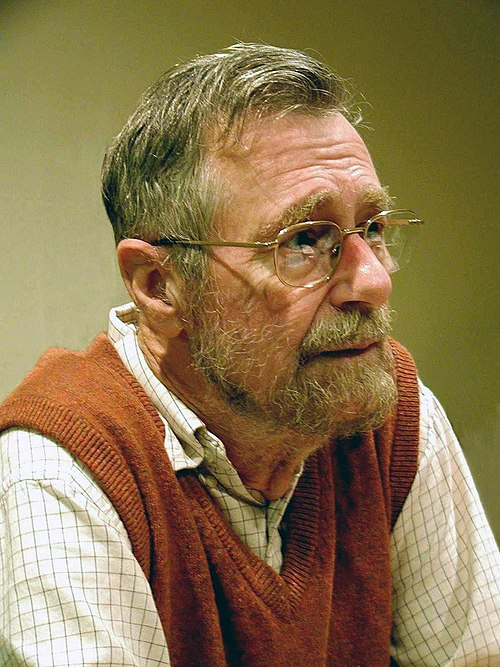
\includegraphics[width=1.04167in,height=\textheight,keepaspectratio]{images/dijkstra.jpg}

Dijkstra 2002

\end{tcolorbox}

\subsubsection{Versuch 3}\label{versuch-3}

\begin{quote}
``Informatik ist die systematische Untersuchung algorithmischer
Prozesse, die Information beschreiben und transformieren: ihre Theorie,
Analyse, Entwurf, Effizienz, Implementierung und Anwendung.'' - Quelle:
ACM / IEEE Computer Science Curricula (z.B. CS2008/CS2013 Report)
\end{quote}

\begin{tcolorbox}[enhanced jigsaw, breakable, coltitle=black, colbacktitle=quarto-callout-tip-color!10!white, colback=white, arc=.35mm, colframe=quarto-callout-tip-color-frame, titlerule=0mm, leftrule=.75mm, title=\textcolor{quarto-callout-tip-color}{\faLightbulb}\hspace{0.5em}{INFO}, toprule=.15mm, bottomtitle=1mm, rightrule=.15mm, bottomrule=.15mm, toptitle=1mm, opacityback=0, left=2mm, opacitybacktitle=0.6]

Die ACM (Association for Computing Machinery, gegründet 1947) ist die
weltweit größte Fachgesellschaft für Informatik. Sie fördert Forschung,
Bildung und professionelle Standards und publiziert mit der Digital
Library zahlreiche Fachzeitschriften sowie Richtlinien (z.B. Curricula,
Code of Ethics). Bedeutend sind ihre Konferenzen und Auszeichnungen wie
der Turing Award

\end{tcolorbox}

\subsubsection{Zusammenfassung}\label{zusammenfassung}

\textbf{Informatik} ist eine interdisziplinäre Wissenschaft, die sich
mit der Analyse von Strukturen beschäftigt. Die ist eine
Strukturwissenschaft. Sie ist verwandt mit der Mathematik, insbesondere
der Logik und der Algebra. Ihre Sprache ist die Mathematik. Gleichzeitig
beschäftigt sich Informatik auch mit dem Entwurf von Artefakten und ist
somit auch eine Ingenieurswissenschaft.

\subsection{2. Einordnung als
Wissenschaft}\label{einordnung-als-wissenschaft}

Die Informatik ist eine \textbf{junge Wissenschaft} (entstanden in den
1960er Jahren) mit:

\textbf{Methodischen Ansätzen:} - \textbf{Empirisch:} Experimente und
Messungen - \textbf{Formal:} Mathematische Beweise und Modelle\\
- \textbf{Konstruktiv:} Entwurf und Implementation von Systemen

\textbf{Interdisziplinäre Verbindungen:} - \textbf{Mathematik:}
Algorithmen, Logik, Statistik - \textbf{Ingenieurswissenschaften:}
Hardware, Systemdesign - \textbf{Naturwissenschaften:} Modellierung,
Simulation - \textbf{Geisteswissenschaften:} Human-Computer Interaction,
Ethik

\subsection{3. Teilgebiete der
Informatik}\label{teilgebiete-der-informatik}

Die Informatik gliedert sich in vier Hauptbereiche, die sich
überschneiden und ergänzen:

\subsubsection{3.1 Theoretische
Informatik}\label{theoretische-informatik}

\textbf{Fokus:} Mathematische Grundlagen der Informatik

\textbf{Kerngebiete:} - \textbf{Algorithmentheorie:} Entwurf und Analyse
von Algorithmen - \textbf{Komplexitätstheorie:} Bewertung des
Ressourcenverbrauchs (Zeit, Speicher) - \textbf{Automatentheorie:}
Mathematische Modelle für Berechnungen - \textbf{Formale Sprachen:}
Grammatiken und Sprachtheorie - \textbf{Berechenbarkeitstheorie:} Was
ist überhaupt algorithmisch lösbar? - \textbf{Logik:} Formale Systeme
für automatisches Schließen

\textbf{Beispielfragen:} - Wie schnell ist ein Sortieralgorithmus?
(O-Notation) - Gibt es Probleme, die prinzipiell unlösbar sind? - Wie
kann man Programmiersprachen formal beschreiben?

\textbf{Bedeutung:} Fundament für alle anderen Bereiche der Informatik

\subsubsection{3.2 Praktische Informatik}\label{praktische-informatik}

\textbf{Fokus:} Methoden und Techniken zur Software-Entwicklung

\textbf{Kerngebiete:} - \textbf{Programmierung:} Implementation von
Algorithmen in verschiedenen Paradigmen - \textbf{Software Engineering:}
Systematische Entwicklung großer Software-Systeme -
\textbf{Datenstrukturen:} Effiziente Organisation und Verwaltung von
Daten - \textbf{Datenbanksysteme:} Persistente und konsistente
Datenverwaltung - \textbf{Compilerbau:} Übersetzung von
Programmiersprachen - \textbf{Betriebssysteme:} Verwaltung von
Hardware-Ressourcen

\textbf{Beispielprojekte:} - Entwicklung einer Web-Anwendung mit
Frontend und Backend - Design einer skalierbaren Datenbank-Architektur -
Implementation eines Interpreters für eine einfache Programmiersprache

\subsubsection{3.3 Technische Informatik}\label{technische-informatik}

\textbf{Fokus:} Hardware und systemnahe Software

\textbf{Kerngebiete:} - \textbf{Rechnerarchitektur:} Aufbau von
Computersystemen (von der CPU bis zum Supercomputer) -
\textbf{Mikrocontroller:} Eingebettete Systeme für spezielle Anwendungen
- \textbf{Betriebssysteme:} Low-Level Systemsoftware -
\textbf{Netzwerktechnik:} Protokolle und Infrastruktur für Kommunikation
- \textbf{Parallelverarbeitung:} Multi-Core und verteilte Systeme -
\textbf{Hardware-Design:} Entwicklung von Prozessoren und Schaltkreisen

\textbf{Anwendungen:} - Internet of Things (IoT) - Vernetzte
Alltagsgegenstände - Autonome Fahrzeuge - Sensorfusion und
Echtzeitverarbeitung - Industrielle Steuerungen - Automatisierung von
Produktionsprozessen - High-Performance Computing - Wissenschaftliche
Simulationen

\subsubsection{3.4 Angewandte Informatik}\label{angewandte-informatik}

\textbf{Fokus:} Informatik in spezifischen Anwendungsdomänen

\textbf{Kerngebiete:}

\begin{itemize}
\tightlist
\item
  \textbf{Künstliche Intelligenz:} Machine Learning, Deep Learning,
  Robotik
\item
  \textbf{Computergrafik:} 2D/3D-Visualisierung, Virtual/Augmented
  Reality
\item
  \textbf{Bioinformatik:} Informatik-Methoden in der Biologie und
  Medizin
\item
  \textbf{Wirtschaftsinformatik:} IT-Lösungen für Unternehmen
\item
  \textbf{Medizininformatik:} IT im Gesundheitswesen
\item
  \textbf{Digitale Medien:} Multimedia-Systeme, Game Development
\item
  \textbf{Human-Computer Interaction:} Benutzerfreundliche Interfaces
\end{itemize}

\textbf{Aktuelle Trends:}

\begin{itemize}
\tightlist
\item
  \textbf{Künstliche Intelligenz:} ChatGPT, autonome Systeme
\item
  \textbf{Internet of Things:} Smart Cities, Industry 4.0
\item
  \textbf{Cloud Computing:} Skalierbare, verteilte Systeme
\item
  \textbf{Blockchain:} Dezentrale, vertrauenslose Systeme
\item
  \textbf{Quantum Computing:} Quantenalgorithmen und -hardware
\end{itemize}

\subsection{4. Begriffe der Informatik}\label{begriffe-der-informatik}

\subsubsection{4.1 Computer}\label{computer}

\textbf{Entymologie} Der Begriff „Computer`` stammt vom lateinischen
„computare`` (zusammenrechnen, berechnen), über englisch „to compute``.
Ursprünglich bezeichnete „computer`` im 17.--19. Jahrhundert eine Person
(oft weiblich), die beruflich Berechnungen ausführte. Mit dem Aufkommen
elektromechanischer und später elektronischer Rechenmaschinen ging die
Bezeichnung auf die Geräte über (spätestens Mitte des 20. Jahrhunderts).
Im Deutschen setzte sich parallel der Begriff „Rechner`` als
sachlich-technische Entsprechung durch. Die Etymologie spiegelt somit
den Wandel vom menschlichen Tätigkeitswort zur Bezeichnung eines
automatisierten Informationsverarbeitungssystems.

\textbf{Computer im Alltag}

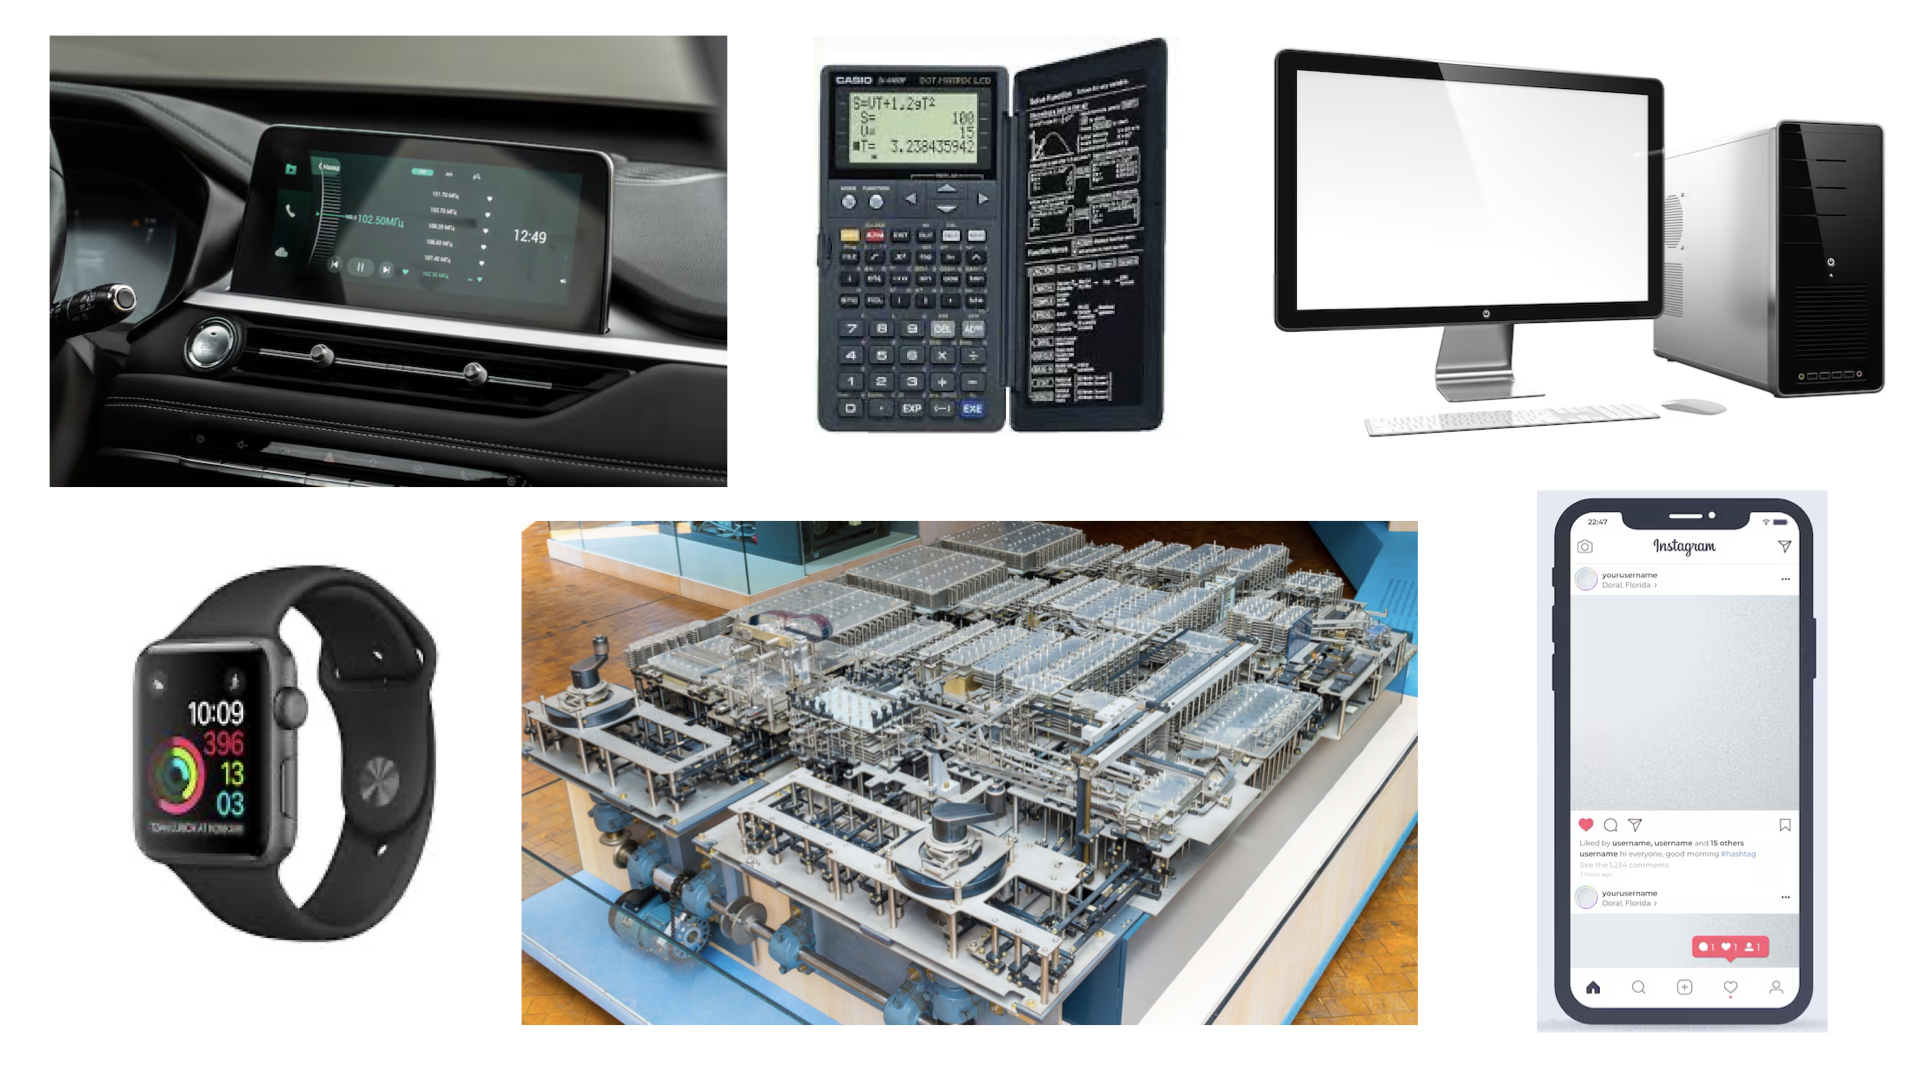
\includegraphics[width=4.16667in,height=\textheight,keepaspectratio]{images/computer.001.jpeg}

\textbf{Eigenschaften} - Universell einsetzbares Gerät zur automatischen
Verarbeitung von Daten. (Quelle: Informatik-Dude) - Prinzipielle
Fähigkeiten und Beschränkungen von idealisierten Computern werden durch
das Automatenmodell der Turingmaschinen beschrieben. - Aufbau nach der
von-Neumann-Architektur.

\textbf{Arbeitsweise} - Eingabe: Daten werden in den Arbeitsspeicher
geladen. - Programm:Abstraktion eines realen Problems in einen
Algorithmus. - Verarbeitung: CPU führt Berechnungen durch. - Ausgabe:
Ergebnisse werden ausgegeben oder gespeichert.

\subsubsection{4.2 Programm}\label{programm}

\begin{tcolorbox}[enhanced jigsaw, breakable, coltitle=black, colbacktitle=quarto-callout-note-color!10!white, colback=white, arc=.35mm, colframe=quarto-callout-note-color-frame, titlerule=0mm, leftrule=.75mm, title=\textcolor{quarto-callout-note-color}{\faInfo}\hspace{0.5em}{Definition}, toprule=.15mm, bottomtitle=1mm, rightrule=.15mm, bottomrule=.15mm, toptitle=1mm, opacityback=0, left=2mm, opacitybacktitle=0.6]

Ein \textbf{Programm} ist ein in einer konkreten Programmiersprache
kodierter Algorithmus, der von einem Computer ausgeführt werden kann.

\end{tcolorbox}

\textbf{Beziehungskette:}

\[
\text{Reales Problem} \rightarrow \text{Abstraktion} \rightarrow \text{Algorithmus}\]
\[
\rightarrow \text{Kodierung} \rightarrow \text{Programm} \rightarrow \text{Ausführung} \Rightarrow \text{Lösung}
\]

\textbf{Eigenschaften von Programmen:} - \textbf{Syntax:}
Grammatikalische Korrektheit nach Sprachregeln - \textbf{Semantik:}
Bedeutung und Verhalten des Programms - \textbf{Pragmatik:} Praktische
Aspekte wie Effizienz, Wartbarkeit, Lesbarkeit

\subsubsection{4.3 Algorithmus}\label{algorithmus}

Zentraler Begriff der Informatik. Er beschreibt eine eindeutige,
schrittweise Vorgehensweise zur Lösung eines Problems und ist
vergleichbar mit einem Kochrezept.

Genauere Bearbeitung später.




\end{document}
